% Options for packages loaded elsewhere
\PassOptionsToPackage{unicode}{hyperref}
\PassOptionsToPackage{hyphens}{url}
%
\documentclass[
]{article}
\usepackage{amsmath,amssymb}
\usepackage{iftex}
\ifPDFTeX
  \usepackage[T1]{fontenc}
  \usepackage[utf8]{inputenc}
  \usepackage{textcomp} % provide euro and other symbols
\else % if luatex or xetex
  \usepackage{unicode-math} % this also loads fontspec
  \defaultfontfeatures{Scale=MatchLowercase}
  \defaultfontfeatures[\rmfamily]{Ligatures=TeX,Scale=1}
\fi
\usepackage{lmodern}
\ifPDFTeX\else
  % xetex/luatex font selection
\fi
% Use upquote if available, for straight quotes in verbatim environments
\IfFileExists{upquote.sty}{\usepackage{upquote}}{}
\IfFileExists{microtype.sty}{% use microtype if available
  \usepackage[]{microtype}
  \UseMicrotypeSet[protrusion]{basicmath} % disable protrusion for tt fonts
}{}
\makeatletter
\@ifundefined{KOMAClassName}{% if non-KOMA class
  \IfFileExists{parskip.sty}{%
    \usepackage{parskip}
  }{% else
    \setlength{\parindent}{0pt}
    \setlength{\parskip}{6pt plus 2pt minus 1pt}}
}{% if KOMA class
  \KOMAoptions{parskip=half}}
\makeatother
\usepackage{xcolor}
\usepackage[margin=1in]{geometry}
\usepackage{color}
\usepackage{fancyvrb}
\newcommand{\VerbBar}{|}
\newcommand{\VERB}{\Verb[commandchars=\\\{\}]}
\DefineVerbatimEnvironment{Highlighting}{Verbatim}{commandchars=\\\{\}}
% Add ',fontsize=\small' for more characters per line
\usepackage{framed}
\definecolor{shadecolor}{RGB}{248,248,248}
\newenvironment{Shaded}{\begin{snugshade}}{\end{snugshade}}
\newcommand{\AlertTok}[1]{\textcolor[rgb]{0.94,0.16,0.16}{#1}}
\newcommand{\AnnotationTok}[1]{\textcolor[rgb]{0.56,0.35,0.01}{\textbf{\textit{#1}}}}
\newcommand{\AttributeTok}[1]{\textcolor[rgb]{0.13,0.29,0.53}{#1}}
\newcommand{\BaseNTok}[1]{\textcolor[rgb]{0.00,0.00,0.81}{#1}}
\newcommand{\BuiltInTok}[1]{#1}
\newcommand{\CharTok}[1]{\textcolor[rgb]{0.31,0.60,0.02}{#1}}
\newcommand{\CommentTok}[1]{\textcolor[rgb]{0.56,0.35,0.01}{\textit{#1}}}
\newcommand{\CommentVarTok}[1]{\textcolor[rgb]{0.56,0.35,0.01}{\textbf{\textit{#1}}}}
\newcommand{\ConstantTok}[1]{\textcolor[rgb]{0.56,0.35,0.01}{#1}}
\newcommand{\ControlFlowTok}[1]{\textcolor[rgb]{0.13,0.29,0.53}{\textbf{#1}}}
\newcommand{\DataTypeTok}[1]{\textcolor[rgb]{0.13,0.29,0.53}{#1}}
\newcommand{\DecValTok}[1]{\textcolor[rgb]{0.00,0.00,0.81}{#1}}
\newcommand{\DocumentationTok}[1]{\textcolor[rgb]{0.56,0.35,0.01}{\textbf{\textit{#1}}}}
\newcommand{\ErrorTok}[1]{\textcolor[rgb]{0.64,0.00,0.00}{\textbf{#1}}}
\newcommand{\ExtensionTok}[1]{#1}
\newcommand{\FloatTok}[1]{\textcolor[rgb]{0.00,0.00,0.81}{#1}}
\newcommand{\FunctionTok}[1]{\textcolor[rgb]{0.13,0.29,0.53}{\textbf{#1}}}
\newcommand{\ImportTok}[1]{#1}
\newcommand{\InformationTok}[1]{\textcolor[rgb]{0.56,0.35,0.01}{\textbf{\textit{#1}}}}
\newcommand{\KeywordTok}[1]{\textcolor[rgb]{0.13,0.29,0.53}{\textbf{#1}}}
\newcommand{\NormalTok}[1]{#1}
\newcommand{\OperatorTok}[1]{\textcolor[rgb]{0.81,0.36,0.00}{\textbf{#1}}}
\newcommand{\OtherTok}[1]{\textcolor[rgb]{0.56,0.35,0.01}{#1}}
\newcommand{\PreprocessorTok}[1]{\textcolor[rgb]{0.56,0.35,0.01}{\textit{#1}}}
\newcommand{\RegionMarkerTok}[1]{#1}
\newcommand{\SpecialCharTok}[1]{\textcolor[rgb]{0.81,0.36,0.00}{\textbf{#1}}}
\newcommand{\SpecialStringTok}[1]{\textcolor[rgb]{0.31,0.60,0.02}{#1}}
\newcommand{\StringTok}[1]{\textcolor[rgb]{0.31,0.60,0.02}{#1}}
\newcommand{\VariableTok}[1]{\textcolor[rgb]{0.00,0.00,0.00}{#1}}
\newcommand{\VerbatimStringTok}[1]{\textcolor[rgb]{0.31,0.60,0.02}{#1}}
\newcommand{\WarningTok}[1]{\textcolor[rgb]{0.56,0.35,0.01}{\textbf{\textit{#1}}}}
\usepackage{graphicx}
\makeatletter
\def\maxwidth{\ifdim\Gin@nat@width>\linewidth\linewidth\else\Gin@nat@width\fi}
\def\maxheight{\ifdim\Gin@nat@height>\textheight\textheight\else\Gin@nat@height\fi}
\makeatother
% Scale images if necessary, so that they will not overflow the page
% margins by default, and it is still possible to overwrite the defaults
% using explicit options in \includegraphics[width, height, ...]{}
\setkeys{Gin}{width=\maxwidth,height=\maxheight,keepaspectratio}
% Set default figure placement to htbp
\makeatletter
\def\fps@figure{htbp}
\makeatother
\setlength{\emergencystretch}{3em} % prevent overfull lines
\providecommand{\tightlist}{%
  \setlength{\itemsep}{0pt}\setlength{\parskip}{0pt}}
\setcounter{secnumdepth}{-\maxdimen} % remove section numbering
\ifLuaTeX
  \usepackage{selnolig}  % disable illegal ligatures
\fi
\usepackage{bookmark}
\IfFileExists{xurl.sty}{\usepackage{xurl}}{} % add URL line breaks if available
\urlstyle{same}
\hypersetup{
  pdftitle={EP10},
  pdfauthor={Grupo 8},
  hidelinks,
  pdfcreator={LaTeX via pandoc}}

\title{EP10}
\author{Grupo 8}
\date{2024-12-10}

\begin{document}
\maketitle

Para este ejercicio usaremos los datos de medidas anatómicas
recolectados por Heinz et al.~(2003) que ya conocimos en el ejercicio
práctico anterior (disponibles en el archivo ``EP09 Datos.csv''). Como
en este case se requiere de una variable dicotómica, vamos a realizar lo
siguiente:

1.- El equipo crea la variable IMC (índice de masa corporal) como el
peso de una persona (en kilogramos) dividida por el cuadrado de su
estatura (en metros). 2.- Si bien esta variable se usa para clasificar a
las personas en varias clases de estado nutricional (bajo peso, normal,
sobrepeso, obesidad, obesidad mórbida), para efectos de este ejercicio,
usaremos dos clases: sobrepeso (IMC ≥ 23,2) y no sobrepeso (IMC
\textless{} 23,2). 3.- El equipo crea la variable dicotómica EN (estado
nutricional) de acuerdo al valor de IMC de cada persona. Ahora podemos
construir un modelo de regresión logística para predecir la variable EN,
de acuerdo con las siguientes instrucciones:

\subsection{1.-Definir la semilla a utilizar, que corresponde a los
últimos cuatro dígitos del RUN (sin considerar el dígito verificador)
del integrante de mayor edad del
equipo.}\label{definir-la-semilla-a-utilizar-que-corresponde-a-los-uxfaltimos-cuatro-duxedgitos-del-run-sin-considerar-el-duxedgito-verificador-del-integrante-de-mayor-edad-del-equipo.}

\begin{Shaded}
\begin{Highlighting}[]
\CommentTok{\#Realizamos la lectura de los datos.}

\NormalTok{datos }\OtherTok{\textless{}{-}} \FunctionTok{read.csv2}\NormalTok{(}\StringTok{"EP09 Datos.csv"}\NormalTok{)}

\CommentTok{\#Definimos la semilla a utilizar}

\FunctionTok{set.seed}\NormalTok{(}\DecValTok{6887}\NormalTok{)}
\end{Highlighting}
\end{Shaded}

\subsection{2.-Seleccionar una muestra de 150 mujeres (si la semilla es
un número par) o 150 hombres (si la semilla es impar), asegurando que la
mitad tenga estado nutricional ``sobrepeso'' y la otra mitad ``no
sobrepeso'' en cada caso. Dividir esta muestra en dos conjuntos: los
datos de 100 personas (50 con EN ``sobrepeso'') para utilizar en la
construcción de los modelos (entramiento) y 50 personas (25 con EN
``sobrepeso'') para poder
evaluarlos.}\label{seleccionar-una-muestra-de-150-mujeres-si-la-semilla-es-un-nuxfamero-par-o-150-hombres-si-la-semilla-es-impar-asegurando-que-la-mitad-tenga-estado-nutricional-sobrepeso-y-la-otra-mitad-no-sobrepeso-en-cada-caso.-dividir-esta-muestra-en-dos-conjuntos-los-datos-de-100-personas-50-con-en-sobrepeso-para-utilizar-en-la-construcciuxf3n-de-los-modelos-entramiento-y-50-personas-25-con-en-sobrepeso-para-poder-evaluarlos.}

\begin{Shaded}
\begin{Highlighting}[]
\CommentTok{\# Librerias a utilizar}
\FunctionTok{library}\NormalTok{(caret) }
\end{Highlighting}
\end{Shaded}

\begin{verbatim}
## Loading required package: ggplot2
\end{verbatim}

\begin{verbatim}
## Loading required package: lattice
\end{verbatim}

\begin{Shaded}
\begin{Highlighting}[]
\FunctionTok{library}\NormalTok{(dplyr) }
\end{Highlighting}
\end{Shaded}

\begin{verbatim}
## 
## Attaching package: 'dplyr'
\end{verbatim}

\begin{verbatim}
## The following objects are masked from 'package:stats':
## 
##     filter, lag
\end{verbatim}

\begin{verbatim}
## The following objects are masked from 'package:base':
## 
##     intersect, setdiff, setequal, union
\end{verbatim}

\begin{Shaded}
\begin{Highlighting}[]
\FunctionTok{library}\NormalTok{(ggpubr)}
\FunctionTok{library}\NormalTok{(pROC)}
\end{Highlighting}
\end{Shaded}

\begin{verbatim}
## Type 'citation("pROC")' for a citation.
\end{verbatim}

\begin{verbatim}
## 
## Attaching package: 'pROC'
\end{verbatim}

\begin{verbatim}
## The following objects are masked from 'package:stats':
## 
##     cov, smooth, var
\end{verbatim}

\begin{Shaded}
\begin{Highlighting}[]
\FunctionTok{library}\NormalTok{(car)  }
\end{Highlighting}
\end{Shaded}

\begin{verbatim}
## Loading required package: carData
\end{verbatim}

\begin{verbatim}
## 
## Attaching package: 'car'
\end{verbatim}

\begin{verbatim}
## The following object is masked from 'package:dplyr':
## 
##     recode
\end{verbatim}

\begin{Shaded}
\begin{Highlighting}[]
\CommentTok{\#Primero creamos la variable IMC para cada persona}
\CommentTok{\#Añadimos la nueva columna IMC a la tabla de datos usando mutate}

\CommentTok{\# Convertimos la altura de centímetros a metros}
\NormalTok{datos }\OtherTok{\textless{}{-}}\NormalTok{ datos }\SpecialCharTok{\%\textgreater{}\%} \FunctionTok{mutate}\NormalTok{(}\AttributeTok{Height =}\NormalTok{ Height }\SpecialCharTok{/} \DecValTok{100}\NormalTok{)}

\CommentTok{\# Calculamos el IMC }
\NormalTok{datos }\OtherTok{\textless{}{-}}\NormalTok{ datos }\SpecialCharTok{\%\textgreater{}\%} \FunctionTok{mutate}\NormalTok{(}\AttributeTok{IMC =}\NormalTok{ Weight }\SpecialCharTok{/}\NormalTok{ (Height}\SpecialCharTok{\^{}}\DecValTok{2}\NormalTok{))}

\CommentTok{\#Segundo creamos la variable EN para cada persona}
\NormalTok{datos }\OtherTok{\textless{}{-}}\NormalTok{ datos }\SpecialCharTok{\%\textgreater{}\%} \FunctionTok{mutate}\NormalTok{(}\AttributeTok{EN =} \FunctionTok{ifelse}\NormalTok{(IMC }\SpecialCharTok{\textgreater{}=} \FloatTok{23.2}\NormalTok{, }\StringTok{"sobrepeso"}\NormalTok{, }\StringTok{"no sobrepeso"}\NormalTok{))}

\CommentTok{\#Seleccionamos la muestra de 150 hombres.}
\NormalTok{muestra\_sobrepeso }\OtherTok{\textless{}{-}}\NormalTok{ datos }\SpecialCharTok{\%\textgreater{}\%} \FunctionTok{filter}\NormalTok{(Gender }\SpecialCharTok{==} \DecValTok{1} \SpecialCharTok{\&}\NormalTok{ EN }\SpecialCharTok{==} \StringTok{"sobrepeso"}\NormalTok{) }\SpecialCharTok{\%\textgreater{}\%} \FunctionTok{sample\_n}\NormalTok{(}\DecValTok{75}\NormalTok{, }\AttributeTok{replace =} \ConstantTok{FALSE}\NormalTok{)}
\NormalTok{muestra\_no\_sobrepeso }\OtherTok{\textless{}{-}}\NormalTok{ datos }\SpecialCharTok{\%\textgreater{}\%} \FunctionTok{filter}\NormalTok{(Gender }\SpecialCharTok{==} \DecValTok{1} \SpecialCharTok{\&}\NormalTok{ EN }\SpecialCharTok{==} \StringTok{"no sobrepeso"}\NormalTok{) }\SpecialCharTok{\%\textgreater{}\%} \FunctionTok{sample\_n}\NormalTok{(}\DecValTok{75}\NormalTok{, }\AttributeTok{replace =} \ConstantTok{FALSE}\NormalTok{)}

\CommentTok{\#Seleccionamos 50 personas sobrepeso y 50 personas no sobrepeso para construir los modelos. }

\NormalTok{muestra\_sobrepeso\_modelo }\OtherTok{\textless{}{-}}\NormalTok{ muestra\_sobrepeso[}\DecValTok{1}\SpecialCharTok{:}\DecValTok{50}\NormalTok{,]}
\NormalTok{muestra\_no\_sobrepeso\_modelo }\OtherTok{\textless{}{-}}\NormalTok{ muestra\_no\_sobrepeso[}\DecValTok{1}\SpecialCharTok{:}\DecValTok{50}\NormalTok{,]}

\CommentTok{\#Seleccionamos 25 personas sobre peso y 25 personas no sobre peso para evaluar los modelos.}

\NormalTok{muestra\_sobrepeso\_evaluar }\OtherTok{\textless{}{-}}\NormalTok{ muestra\_sobrepeso[}\DecValTok{51}\SpecialCharTok{:}\DecValTok{75}\NormalTok{,]}
\NormalTok{muestra\_no\_sobrepeso\_evaluar }\OtherTok{\textless{}{-}}\NormalTok{ muestra\_no\_sobrepeso[}\DecValTok{51}\SpecialCharTok{:}\DecValTok{75}\NormalTok{,]}

\CommentTok{\# Combinar los conjuntos de entrenamiento}
\NormalTok{muestra\_entrenamiento }\OtherTok{\textless{}{-}} \FunctionTok{bind\_rows}\NormalTok{(muestra\_sobrepeso\_modelo, muestra\_no\_sobrepeso\_modelo)}

\CommentTok{\# Combinar los conjuntos de prueba}
\NormalTok{muestra\_prueba }\OtherTok{\textless{}{-}} \FunctionTok{bind\_rows}\NormalTok{(muestra\_sobrepeso\_evaluar, muestra\_no\_sobrepeso\_evaluar)}
\end{Highlighting}
\end{Shaded}

\subsection{3.-Recordar las ocho posibles variables predictoras
seleccionadas de forma aleatoria en el ejercicio
anterior.}\label{recordar-las-ocho-posibles-variables-predictoras-seleccionadas-de-forma-aleatoria-en-el-ejercicio-anterior.}

\begin{Shaded}
\begin{Highlighting}[]
\CommentTok{\#Aplicando filtro para obtener solo las 8 variables que obtuvimos aleatoriamente}
\CommentTok{\# Guardar los nombres de las variables seleccionadas}
\NormalTok{nombres\_variables }\OtherTok{\textless{}{-}} \FunctionTok{c}\NormalTok{(}\StringTok{"Knees.diameter"}\NormalTok{, }\StringTok{"Gender"}\NormalTok{, }\StringTok{"Chest.Girth"}\NormalTok{, }
                       \StringTok{"Ankle.Minimum.Girth"}\NormalTok{, }\StringTok{"Age"}\NormalTok{, }
                       \StringTok{"Navel.Girth"}\NormalTok{, }\StringTok{"Hip.Girth"}\NormalTok{, }
                       \StringTok{"Elbows.diameter"}\NormalTok{)}

\CommentTok{\# Seleccionar las variables deseadas}
\NormalTok{variables\_seleccionadas }\OtherTok{\textless{}{-}} \FunctionTok{subset}\NormalTok{(datos, }\AttributeTok{select =} \FunctionTok{c}\NormalTok{(}\StringTok{"Knees.diameter"}\NormalTok{, }\StringTok{"Gender"}\NormalTok{, }\StringTok{"Chest.Girth"}\NormalTok{, }
                                                      \StringTok{"Ankle.Minimum.Girth"}\NormalTok{, }\StringTok{"Age"}\NormalTok{, }
                                                      \StringTok{"Navel.Girth"}\NormalTok{, }\StringTok{"Hip.Girth"}\NormalTok{, }
                                                      \StringTok{"Elbows.diameter"}\NormalTok{))}
\end{Highlighting}
\end{Shaded}

\subsection{4.-Seleccionar, de las otras variables, una que el equipo
considere que podría ser útil para predecir la clase EN, justificando
bien esta selección (idealmente con
literatura).}\label{seleccionar-de-las-otras-variables-una-que-el-equipo-considere-que-podruxeda-ser-uxfatil-para-predecir-la-clase-en-justificando-bien-esta-selecciuxf3n-idealmente-con-literatura.}

Siendo EN la variable dicotómica estado nutricional seleccionaremos la
variables Waist Girth (que es la circunferencia de la cintura) para
predecir el estado nutricional ya que ayuda a evaluar la distribución de
la grasa corporal y puede ayudar a identificar la obesidad, siendo las
personas que tengan una circunferencia elevada probablemente las que
tengan un IMC igualmente elevado\\
-
\url{https://scielo.isciii.es/scielo.php?script=sci_arttext&pid=S0212-16112010000900009}\\
-
\url{https://ojs.unemi.edu.ec/index.php/facsalud-unemi/article/view/1463}

\begin{Shaded}
\begin{Highlighting}[]
\CommentTok{\# Obtenemos los nombres de todas las columnas en el conjunto de datos original}
\NormalTok{nombres\_completos }\OtherTok{\textless{}{-}} \FunctionTok{names}\NormalTok{(datos)}

\CommentTok{\# Identificamos las variables restantes}
\NormalTok{variables\_restantes }\OtherTok{\textless{}{-}} \FunctionTok{setdiff}\NormalTok{(nombres\_completos, nombres\_variables)}

\CommentTok{\#por si hay que quitar height y weight igual que en EP09}
\CommentTok{\#variables\_restantes \textless{}{-} setdiff(variables\_restantes, c("Height", "Weight"))}

\CommentTok{\# Como queremos predecir estas variables, deberiamos quitarlas del conjunto de datos}
\NormalTok{variables\_restantes }\OtherTok{\textless{}{-}} \FunctionTok{setdiff}\NormalTok{(variables\_restantes, }\FunctionTok{c}\NormalTok{(}\StringTok{"EN"}\NormalTok{, }\StringTok{"IMC"}\NormalTok{))}


\CommentTok{\# Creamos un arreglo que tenga las variables restantes del conjunto de datos original}
\NormalTok{datos\_restantes }\OtherTok{\textless{}{-}}\NormalTok{ datos[, variables\_restantes]}



\NormalTok{variables\_restantes}
\end{Highlighting}
\end{Shaded}

\begin{verbatim}
##  [1] "Biacromial.diameter"     "Biiliac.diameter"       
##  [3] "Bitrochanteric.diameter" "Chest.depth"            
##  [5] "Chest.diameter"          "Wrists.diameter"        
##  [7] "Ankles.diameter"         "Shoulder.Girth"         
##  [9] "Waist.Girth"             "Thigh.Girth"            
## [11] "Bicep.Girth"             "Forearm.Girth"          
## [13] "Knee.Girth"              "Calf.Maximum.Girth"     
## [15] "Wrist.Minimum.Girth"     "Weight"                 
## [17] "Height"
\end{verbatim}

\subsection{5.-Usando el entorno R, construir un modelo de regresión
logística con el predictor seleccionado en el paso anterior y utilizando
de la muestra
obtenida.}\label{usando-el-entorno-r-construir-un-modelo-de-regresiuxf3n-loguxedstica-con-el-predictor-seleccionado-en-el-paso-anterior-y-utilizando-de-la-muestra-obtenida.}

\begin{Shaded}
\begin{Highlighting}[]
\CommentTok{\#logit indica que usamos regresion logistica}
\FunctionTok{set.seed}\NormalTok{(}\DecValTok{6887}\NormalTok{)}

\CommentTok{\# Sacamos EN y lo convertimos en factor}
\NormalTok{muestra\_entrenamiento }\OtherTok{\textless{}{-}}\NormalTok{ muestra\_entrenamiento }\SpecialCharTok{\%\textgreater{}\%}
    \FunctionTok{mutate}\NormalTok{(}\AttributeTok{EN =} \FunctionTok{factor}\NormalTok{(EN, }\AttributeTok{levels =} \FunctionTok{c}\NormalTok{(}\StringTok{"no sobrepeso"}\NormalTok{, }\StringTok{"sobrepeso"}\NormalTok{)))}

\CommentTok{\#Ajustar modelo.}
\NormalTok{modelo }\OtherTok{\textless{}{-}} \FunctionTok{glm}\NormalTok{(EN }\SpecialCharTok{\textasciitilde{}}\NormalTok{ Waist.Girth, }\AttributeTok{family =} \FunctionTok{binomial}\NormalTok{(}\AttributeTok{link =} \StringTok{"logit"}\NormalTok{), }\AttributeTok{data =}\NormalTok{ muestra\_entrenamiento)}

\FunctionTok{print}\NormalTok{(}\FunctionTok{summary}\NormalTok{ (modelo))}
\end{Highlighting}
\end{Shaded}

\begin{verbatim}
## 
## Call:
## glm(formula = EN ~ Waist.Girth, family = binomial(link = "logit"), 
##     data = muestra_entrenamiento)
## 
## Coefficients:
##              Estimate Std. Error z value Pr(>|z|)    
## (Intercept) -19.36784    3.93084  -4.927 8.34e-07 ***
## Waist.Girth   0.23649    0.04816   4.911 9.08e-07 ***
## ---
## Signif. codes:  0 '***' 0.001 '**' 0.01 '*' 0.05 '.' 0.1 ' ' 1
## 
## (Dispersion parameter for binomial family taken to be 1)
## 
##     Null deviance: 138.629  on 99  degrees of freedom
## Residual deviance:  94.111  on 98  degrees of freedom
## AIC: 98.111
## 
## Number of Fisher Scoring iterations: 5
\end{verbatim}

\begin{Shaded}
\begin{Highlighting}[]
\CommentTok{\#Evaluar el modelo con el conjunto de entrenamiento.}
\NormalTok{probs\_ent }\OtherTok{\textless{}{-}} \FunctionTok{fitted}\NormalTok{(modelo)}

\CommentTok{\# Graficar curva ROC, indicando AUC obtenido.}
\NormalTok{ROC\_ent }\OtherTok{\textless{}{-}} \FunctionTok{roc}\NormalTok{(muestra\_entrenamiento[[}\StringTok{"EN"}\NormalTok{]], probs\_ent) }
\end{Highlighting}
\end{Shaded}

\begin{verbatim}
## Setting levels: control = no sobrepeso, case = sobrepeso
\end{verbatim}

\begin{verbatim}
## Setting direction: controls < cases
\end{verbatim}

\begin{Shaded}
\begin{Highlighting}[]
\NormalTok{texto\_ent}\OtherTok{\textless{}{-}} \FunctionTok{sprintf}\NormalTok{(}\StringTok{"AUC = \%.2f"}\NormalTok{, ROC\_ent[[}\StringTok{"auc"}\NormalTok{]])}
\NormalTok{g\_roc\_ent }\OtherTok{\textless{}{-}} \FunctionTok{ggroc}\NormalTok{(ROC\_ent, }\AttributeTok{color =} \DecValTok{2}\NormalTok{)}
\NormalTok{g\_roc\_ent }\OtherTok{\textless{}{-}}\NormalTok{ g\_roc\_ent }\SpecialCharTok{+} \FunctionTok{geom\_segment}\NormalTok{(}\FunctionTok{aes}\NormalTok{(}\AttributeTok{x =} \DecValTok{1}\NormalTok{, }\AttributeTok{xend =} \DecValTok{0}\NormalTok{, }\AttributeTok{y =}
                                            \DecValTok{0}\NormalTok{, }\AttributeTok{yend=} \DecValTok{1}\NormalTok{), }\AttributeTok{linetype =} \StringTok{"dashed"}\NormalTok{)}

\NormalTok{g\_roc\_ent }\OtherTok{\textless{}{-}}\NormalTok{ g\_roc\_ent }\SpecialCharTok{+} \FunctionTok{annotate}\NormalTok{(}\StringTok{"text"}\NormalTok{, }\AttributeTok{x=} \FloatTok{0.3}\NormalTok{, }\AttributeTok{y=} \FloatTok{0.3}\NormalTok{,}
                                  \AttributeTok{label =}\NormalTok{ texto\_ent)}
\NormalTok{g\_roc\_ent }\OtherTok{\textless{}{-}}\NormalTok{ g\_roc\_ent }\SpecialCharTok{+} \FunctionTok{theme\_pubr}\NormalTok{ ()}
\FunctionTok{print}\NormalTok{(g\_roc\_ent)}
\end{Highlighting}
\end{Shaded}

\begin{verbatim}
## Warning in geom_segment(aes(x = 1, xend = 0, y = 0, yend = 1), linetype = "dashed"): All aesthetics have length 1, but the data has 81 rows.
## i Please consider using `annotate()` or provide this layer with data containing
##   a single row.
\end{verbatim}

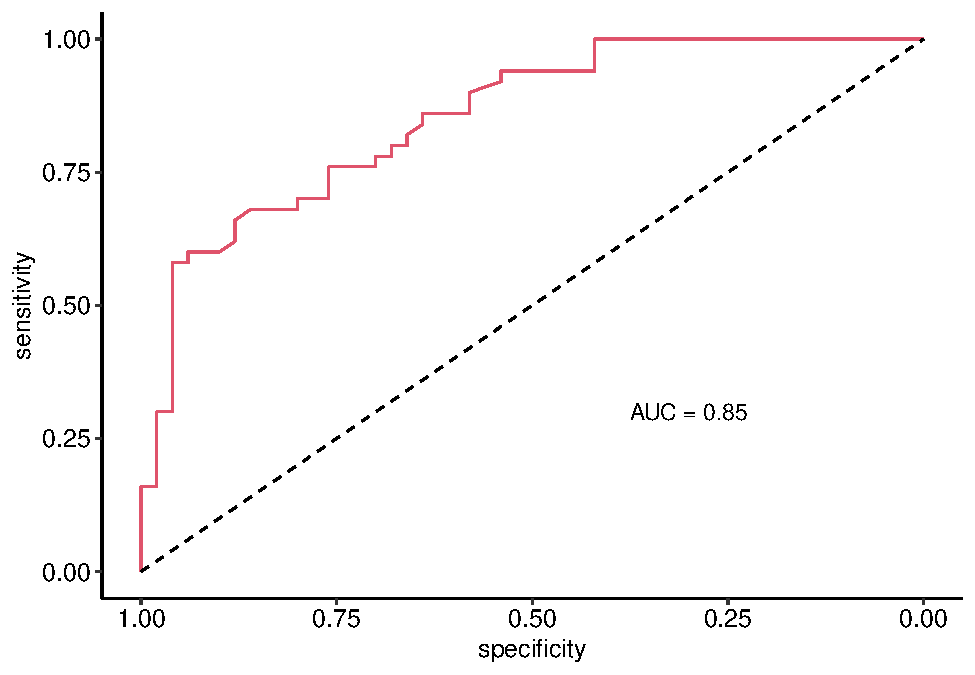
\includegraphics{ep10_files/figure-latex/unnamed-chunk-5-1.pdf}

\begin{Shaded}
\begin{Highlighting}[]
\CommentTok{\#Obtener las predicciones.}
\NormalTok{umbral }\OtherTok{\textless{}{-}} \FloatTok{0.5}
\NormalTok{preds\_ent }\OtherTok{\textless{}{-}} \FunctionTok{sapply}\NormalTok{(probs\_ent,}
                    \ControlFlowTok{function}\NormalTok{(p) }\FunctionTok{ifelse}\NormalTok{(p }\SpecialCharTok{\textgreater{}=}\NormalTok{ umbral, }\StringTok{"sobrepeso"}\NormalTok{, }\StringTok{"no sobrepeso"}\NormalTok{)) }
\NormalTok{preds\_ent }\OtherTok{\textless{}{-}} \FunctionTok{factor}\NormalTok{(preds\_ent, }\AttributeTok{levels =} \FunctionTok{c}\NormalTok{(}\StringTok{"no sobrepeso"}\NormalTok{, }\StringTok{"sobrepeso"}\NormalTok{))}

\CommentTok{\# Obtener y mostrar estadísticas de clasificación en datos de entrenamiento. }
\NormalTok{mat\_conf\_ent }\OtherTok{\textless{}{-}} \FunctionTok{confusionMatrix}\NormalTok{(preds\_ent, muestra\_entrenamiento[[}\StringTok{"EN"}\NormalTok{]],}
                                \AttributeTok{positive =} \StringTok{"sobrepeso"}\NormalTok{)}
\FunctionTok{cat}\NormalTok{(}\StringTok{"}\SpecialCharTok{\textbackslash{}n\textbackslash{}n}\StringTok{Evaluación del modelo (cjto. de entrenamiento): }\SpecialCharTok{\textbackslash{}n}\StringTok{"}\NormalTok{)}
\end{Highlighting}
\end{Shaded}

\begin{verbatim}
## 
## 
## Evaluación del modelo (cjto. de entrenamiento):
\end{verbatim}

\begin{Shaded}
\begin{Highlighting}[]
\FunctionTok{cat}\NormalTok{(}\StringTok{"{-}{-}{-}{-}{-}{-}{-}{-}{-}{-}{-}{-}{-}{-}{-}{-}{-}}\SpecialCharTok{\textbackslash{}n}\StringTok{"}\NormalTok{)}
\end{Highlighting}
\end{Shaded}

\begin{verbatim}
## -----------------
\end{verbatim}

\begin{Shaded}
\begin{Highlighting}[]
\FunctionTok{print}\NormalTok{(mat\_conf\_ent[[}\StringTok{"table"}\NormalTok{]])}
\end{Highlighting}
\end{Shaded}

\begin{verbatim}
##               Reference
## Prediction     no sobrepeso sobrepeso
##   no sobrepeso           38        12
##   sobrepeso              12        38
\end{verbatim}

\begin{Shaded}
\begin{Highlighting}[]
\FunctionTok{cat}\NormalTok{ (}\StringTok{"}\SpecialCharTok{\textbackslash{}n}\StringTok{"}\NormalTok{)}
\end{Highlighting}
\end{Shaded}

\begin{Shaded}
\begin{Highlighting}[]
\FunctionTok{cat}\NormalTok{(}\FunctionTok{sprintf}\NormalTok{(}\StringTok{" Exactitud: \%.3f}\SpecialCharTok{\textbackslash{}n}\StringTok{"}\NormalTok{, mat\_conf\_ent [[}\StringTok{"overall"}\NormalTok{]][}\StringTok{"Accuracy"}\NormalTok{]))}
\end{Highlighting}
\end{Shaded}

\begin{verbatim}
##  Exactitud: 0.760
\end{verbatim}

\begin{Shaded}
\begin{Highlighting}[]
\FunctionTok{cat}\NormalTok{(}\FunctionTok{sprintf}\NormalTok{(}\StringTok{" Sensibilidad: \%.3f}\SpecialCharTok{\textbackslash{}n}\StringTok{"}\NormalTok{, mat\_conf\_ent[[}\StringTok{"byClass"}\NormalTok{]][}\StringTok{"Sensitivity"}\NormalTok{]))}
\end{Highlighting}
\end{Shaded}

\begin{verbatim}
##  Sensibilidad: 0.760
\end{verbatim}

\begin{Shaded}
\begin{Highlighting}[]
\FunctionTok{cat}\NormalTok{(}\FunctionTok{sprintf}\NormalTok{(}\StringTok{"Especificidad: \%.3f}\SpecialCharTok{\textbackslash{}n}\StringTok{"}\NormalTok{, mat\_conf\_ent [[}\StringTok{"byClass"}\NormalTok{]][}\StringTok{"Specificity"}\NormalTok{]))}
\end{Highlighting}
\end{Shaded}

\begin{verbatim}
## Especificidad: 0.760
\end{verbatim}

\begin{Shaded}
\begin{Highlighting}[]
\CommentTok{\# Evaluar el modelo con el conjunto de prueba.}
\NormalTok{probs\_pru }\OtherTok{\textless{}{-}} \FunctionTok{predict}\NormalTok{(modelo, muestra\_prueba, }\AttributeTok{type=}\StringTok{"response"}\NormalTok{)}

\CommentTok{\# Lo convertimos en factores para que sea coherente con la muestra anterior}
\NormalTok{muestra\_prueba }\OtherTok{\textless{}{-}}\NormalTok{ muestra\_prueba }\SpecialCharTok{\%\textgreater{}\%}
    \FunctionTok{mutate}\NormalTok{(}\AttributeTok{EN =} \FunctionTok{factor}\NormalTok{(EN, }\AttributeTok{levels =} \FunctionTok{c}\NormalTok{(}\StringTok{"no sobrepeso"}\NormalTok{, }\StringTok{"sobrepeso"}\NormalTok{)))}

\CommentTok{\# Graficar curva ROC, indicando AUC obtenido.}
\NormalTok{ROC\_pru}\OtherTok{\textless{}{-}} \FunctionTok{roc}\NormalTok{(muestra\_prueba[[}\StringTok{"EN"}\NormalTok{]], probs\_pru)}
\end{Highlighting}
\end{Shaded}

\begin{verbatim}
## Setting levels: control = no sobrepeso, case = sobrepeso
## Setting direction: controls < cases
\end{verbatim}

\begin{Shaded}
\begin{Highlighting}[]
\NormalTok{texto\_pru }\OtherTok{\textless{}{-}} \FunctionTok{sprintf}\NormalTok{(}\StringTok{"AUC=  \%.2f"}\NormalTok{, ROC\_pru[[}\StringTok{"auc"}\NormalTok{]]) }
\NormalTok{g\_roc\_pru }\OtherTok{\textless{}{-}} \FunctionTok{ggroc}\NormalTok{(ROC\_pru, }\AttributeTok{color =} \DecValTok{2}\NormalTok{)}
\NormalTok{g\_roc\_pru }\OtherTok{\textless{}{-}}\NormalTok{ g\_roc\_pru }\SpecialCharTok{+} \FunctionTok{geom\_segment}\NormalTok{(}\FunctionTok{aes}\NormalTok{(}\AttributeTok{x =} \DecValTok{1}\NormalTok{, }\AttributeTok{xend =} \DecValTok{0}\NormalTok{, }
                                          \AttributeTok{y=}\DecValTok{0}\NormalTok{, }\AttributeTok{yend=} \DecValTok{1}\NormalTok{),}
                                      \AttributeTok{linetype =}\StringTok{"dashed"}\NormalTok{)}

\NormalTok{g\_roc\_pru }\OtherTok{\textless{}{-}}\NormalTok{ g\_roc\_pru }\SpecialCharTok{+} \FunctionTok{annotate}\NormalTok{(}\StringTok{"text"}\NormalTok{, }\AttributeTok{x=} \FloatTok{0.3}\NormalTok{, }\AttributeTok{y=} \FloatTok{0.3}\NormalTok{, }\AttributeTok{label =}\NormalTok{texto\_pru) }
\NormalTok{g\_roc\_pru }\OtherTok{\textless{}{-}}\NormalTok{ g\_roc\_pru}\SpecialCharTok{+}\FunctionTok{theme\_pubr}\NormalTok{()}
\FunctionTok{print}\NormalTok{(g\_roc\_pru)}
\end{Highlighting}
\end{Shaded}

\begin{verbatim}
## Warning in geom_segment(aes(x = 1, xend = 0, y = 0, yend = 1), linetype = "dashed"): All aesthetics have length 1, but the data has 45 rows.
## i Please consider using `annotate()` or provide this layer with data containing
##   a single row.
\end{verbatim}

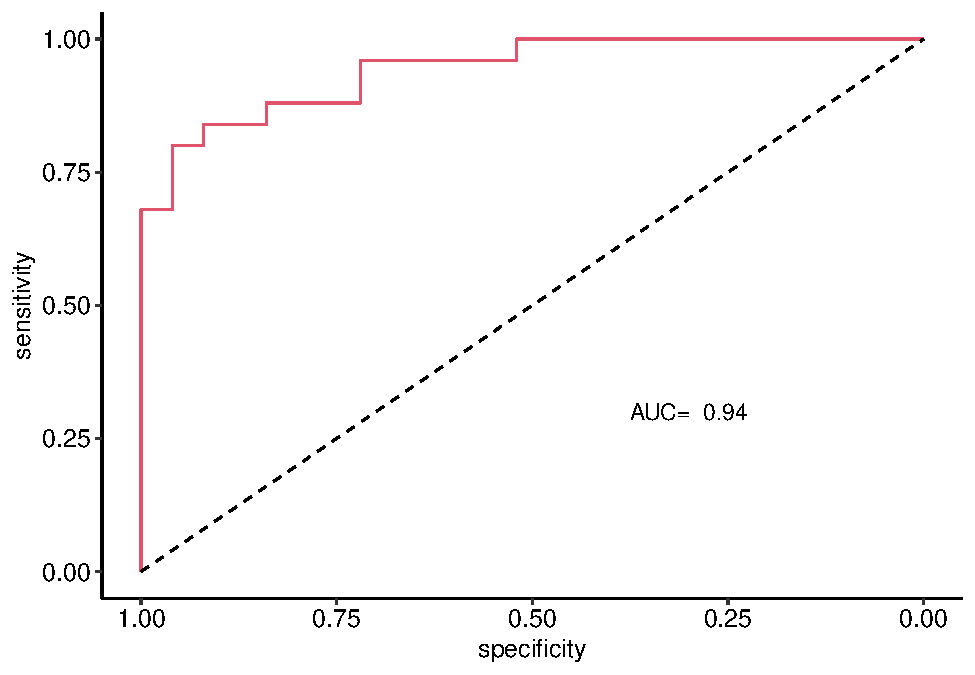
\includegraphics{ep10_files/figure-latex/unnamed-chunk-5-2.pdf}

\begin{Shaded}
\begin{Highlighting}[]
\CommentTok{\# Obtener las predicciones (con el mismo umbral). }
\NormalTok{preds\_pru }\OtherTok{\textless{}{-}} \FunctionTok{sapply}\NormalTok{(probs\_pru,}
                    \ControlFlowTok{function}\NormalTok{(p) }\FunctionTok{ifelse}\NormalTok{(p }\SpecialCharTok{\textgreater{}=}\NormalTok{ umbral, }\StringTok{"sobrepeso"}\NormalTok{, }\StringTok{"no sobrepeso"}\NormalTok{)) }
\NormalTok{preds\_pru }\OtherTok{\textless{}{-}} \FunctionTok{factor}\NormalTok{(preds\_pru, }\AttributeTok{levels =} \FunctionTok{c}\NormalTok{(}\StringTok{"no sobrepeso"}\NormalTok{, }\StringTok{"sobrepeso"}\NormalTok{))}

\CommentTok{\# Obtener y mostrar estadísticas de clasificación en datos de prueba. }
\NormalTok{mat\_conf\_pru }\OtherTok{\textless{}{-}} \FunctionTok{confusionMatrix}\NormalTok{(preds\_pru, muestra\_prueba[[}\StringTok{"EN"}\NormalTok{]],}
                                \AttributeTok{positive=}\StringTok{"sobrepeso"}\NormalTok{)}
\FunctionTok{cat}\NormalTok{(}\StringTok{"}\SpecialCharTok{\textbackslash{}n\textbackslash{}n}\StringTok{Evaluación del modelo (cjto. de prueba): }\SpecialCharTok{\textbackslash{}n}\StringTok{"}\NormalTok{)}
\end{Highlighting}
\end{Shaded}

\begin{verbatim}
## 
## 
## Evaluación del modelo (cjto. de prueba):
\end{verbatim}

\begin{Shaded}
\begin{Highlighting}[]
\FunctionTok{cat}\NormalTok{ (}\StringTok{"{-}{-}{-}{-}{-}{-}{-}{-}{-}{-}{-}{-}}\SpecialCharTok{\textbackslash{}n}\StringTok{"}\NormalTok{)}
\end{Highlighting}
\end{Shaded}

\begin{verbatim}
## ------------
\end{verbatim}

\begin{Shaded}
\begin{Highlighting}[]
\FunctionTok{print}\NormalTok{(mat\_conf\_pru [[}\StringTok{"table"}\NormalTok{]])}
\end{Highlighting}
\end{Shaded}

\begin{verbatim}
##               Reference
## Prediction     no sobrepeso sobrepeso
##   no sobrepeso           23         5
##   sobrepeso               2        20
\end{verbatim}

\begin{Shaded}
\begin{Highlighting}[]
\FunctionTok{cat}\NormalTok{(}\StringTok{"}\SpecialCharTok{\textbackslash{}n}\StringTok{"}\NormalTok{)}
\end{Highlighting}
\end{Shaded}

\begin{Shaded}
\begin{Highlighting}[]
\FunctionTok{cat}\NormalTok{(}\FunctionTok{sprintf}\NormalTok{(}\StringTok{" Exactitud: \%.3f}\SpecialCharTok{\textbackslash{}n}\StringTok{"}\NormalTok{, mat\_conf\_pru [[}\StringTok{"overall"}\NormalTok{]][}\StringTok{"Accuracy"}\NormalTok{])) }
\end{Highlighting}
\end{Shaded}

\begin{verbatim}
##  Exactitud: 0.860
\end{verbatim}

\begin{Shaded}
\begin{Highlighting}[]
\FunctionTok{cat}\NormalTok{(}\FunctionTok{sprintf}\NormalTok{(}\StringTok{" Sensibilidad: \%.3f}\SpecialCharTok{\textbackslash{}n}\StringTok{"}\NormalTok{, mat\_conf\_pru [[}\StringTok{"byClass"}\NormalTok{]][}\StringTok{"Sensitivity"}\NormalTok{]))}
\end{Highlighting}
\end{Shaded}

\begin{verbatim}
##  Sensibilidad: 0.800
\end{verbatim}

\begin{Shaded}
\begin{Highlighting}[]
\FunctionTok{cat}\NormalTok{(}\FunctionTok{sprintf}\NormalTok{(}\StringTok{"Especificidad: \%.3f}\SpecialCharTok{\textbackslash{}n}\StringTok{"}\NormalTok{, mat\_conf\_pru [[}\StringTok{"byClass"}\NormalTok{]][}\StringTok{"Specificity"}\NormalTok{]))}
\end{Highlighting}
\end{Shaded}

\begin{verbatim}
## Especificidad: 0.920
\end{verbatim}

\begin{Shaded}
\begin{Highlighting}[]
\CommentTok{\# Evaluar la linealidad entre predictor y respuesta transformada}
\NormalTok{datos\_lin }\OtherTok{\textless{}{-}}\NormalTok{ muestra\_entrenamiento }\SpecialCharTok{\%\textgreater{}\%}
    \FunctionTok{select}\NormalTok{(Waist.Girth) }\SpecialCharTok{\%\textgreater{}\%}
    \FunctionTok{mutate}\NormalTok{(}\AttributeTok{Logit =} \FunctionTok{log}\NormalTok{(}\FunctionTok{fitted}\NormalTok{(modelo)}\SpecialCharTok{/}\NormalTok{(}\DecValTok{1}\SpecialCharTok{{-}}\FunctionTok{fitted}\NormalTok{(modelo))))}

\NormalTok{p\_lin }\OtherTok{\textless{}{-}} \FunctionTok{ggscatter}\NormalTok{(datos\_lin, }\AttributeTok{x =} \StringTok{"Waist.Girth"}\NormalTok{, }\AttributeTok{y =} \StringTok{"Logit"}\NormalTok{,}
                   \AttributeTok{add =} \StringTok{"reg.line"}\NormalTok{, }\AttributeTok{add.params =} \FunctionTok{list}\NormalTok{(}\AttributeTok{color =} \StringTok{"blue"}\NormalTok{))}
\NormalTok{p\_lin }\OtherTok{\textless{}{-}}\NormalTok{ p\_lin }\SpecialCharTok{+} \FunctionTok{labs}\NormalTok{(}\AttributeTok{x =} \StringTok{"Circunferencia de cintura"}\NormalTok{, }
                      \AttributeTok{y =} \StringTok{"Logit (EN)"}\NormalTok{)}
\FunctionTok{print}\NormalTok{(p\_lin)}
\end{Highlighting}
\end{Shaded}

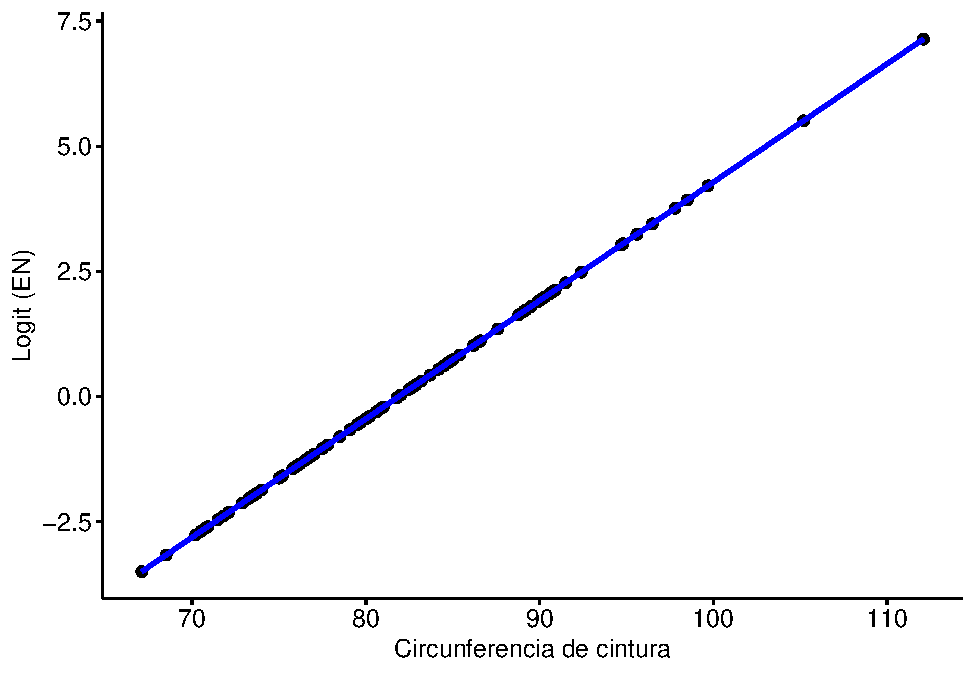
\includegraphics{ep10_files/figure-latex/unnamed-chunk-5-3.pdf}

\begin{Shaded}
\begin{Highlighting}[]
\CommentTok{\# Evaluar independencia de residuos}
\NormalTok{dwtest }\OtherTok{\textless{}{-}} \FunctionTok{durbinWatsonTest}\NormalTok{(modelo)}
\FunctionTok{cat}\NormalTok{(}\StringTok{"}\SpecialCharTok{\textbackslash{}n}\StringTok{Prueba de independencia de residuos:}\SpecialCharTok{\textbackslash{}n}\StringTok{"}\NormalTok{)}
\end{Highlighting}
\end{Shaded}

\begin{verbatim}
## 
## Prueba de independencia de residuos:
\end{verbatim}

\begin{Shaded}
\begin{Highlighting}[]
\FunctionTok{print}\NormalTok{(dwtest)}
\end{Highlighting}
\end{Shaded}

\begin{verbatim}
##  lag Autocorrelation D-W Statistic p-value
##    1       0.7323669     0.5319008       0
##  Alternative hypothesis: rho != 0
\end{verbatim}

\begin{Shaded}
\begin{Highlighting}[]
\CommentTok{\# Evaluar normalidad de residuos}
\NormalTok{residuos\_estand }\OtherTok{\textless{}{-}} \FunctionTok{rstandard}\NormalTok{(modelo)}
\FunctionTok{qqnorm}\NormalTok{(residuos\_estand)}
\FunctionTok{qqline}\NormalTok{(residuos\_estand)}
\end{Highlighting}
\end{Shaded}

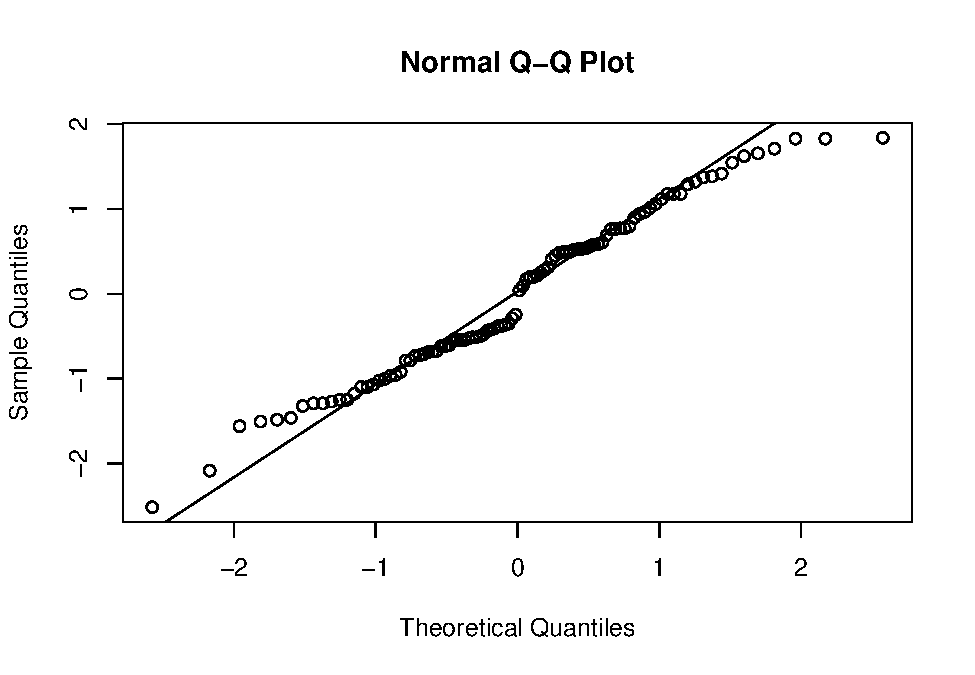
\includegraphics{ep10_files/figure-latex/unnamed-chunk-5-4.pdf}

\begin{Shaded}
\begin{Highlighting}[]
\CommentTok{\# Identificar casos influyentes}
\NormalTok{infl }\OtherTok{\textless{}{-}} \FunctionTok{influence.measures}\NormalTok{(modelo)}
\NormalTok{casos\_influyentes }\OtherTok{\textless{}{-}} \FunctionTok{which}\NormalTok{(}\FunctionTok{apply}\NormalTok{(infl}\SpecialCharTok{$}\NormalTok{is.inf, }\DecValTok{1}\NormalTok{, any))}
\FunctionTok{cat}\NormalTok{(}\StringTok{"}\SpecialCharTok{\textbackslash{}n}\StringTok{Casos influyentes:}\SpecialCharTok{\textbackslash{}n}\StringTok{"}\NormalTok{)}
\end{Highlighting}
\end{Shaded}

\begin{verbatim}
## 
## Casos influyentes:
\end{verbatim}

\begin{Shaded}
\begin{Highlighting}[]
\FunctionTok{print}\NormalTok{(}\FunctionTok{rownames}\NormalTok{(infl}\SpecialCharTok{$}\NormalTok{infmat)[casos\_influyentes])}
\end{Highlighting}
\end{Shaded}

\begin{verbatim}
## [1] "77"
\end{verbatim}

Se ha creado un modelo de regresión logística con variable dependiente
EN y waist girth como variable independiente. Con la matriz de confusión
con el conjunto de entramiento se han predicho a 38 personas con ``no
sobrepeso'' correctamente, mientras 12 han sido incorrectas. Igualmente
se han predicho se han predicho a 38 personas con ``sobrepeso''
correctamente, mientras 12 han sido incorrectas.

Con la matriz del conjunto de prueba se han predicho a 23 personas con
``no sobrepeso'' correctamente, mientras 5 han sido incorrectas.
Igualmente se han predicho se han predicho a 20 personas con
``sobrepeso'' correctamente, mientras 2 han sido incorrectas.

\subsection{6.-Usando estas herramientas para la exploración de modelos
del entorno R1, buscar entre dos y cinco predictores de entre las
variables seleccionadas al azar, recordadas en el punto 3, para agregar
al modelo obtenido en el paso
5.}\label{usando-estas-herramientas-para-la-exploraciuxf3n-de-modelos-del-entorno-r1-buscar-entre-dos-y-cinco-predictores-de-entre-las-variables-seleccionadas-al-azar-recordadas-en-el-punto-3-para-agregar-al-modelo-obtenido-en-el-paso-5.}

\begin{Shaded}
\begin{Highlighting}[]
\CommentTok{\# Primero veamos qué pasa al agregar cada una de las variables seleccionadas al modelo actual}
\FunctionTok{cat}\NormalTok{(}\StringTok{"Single term additions}\SpecialCharTok{\textbackslash{}n}\StringTok{"}\NormalTok{)}
\end{Highlighting}
\end{Shaded}

\begin{verbatim}
## Single term additions
\end{verbatim}

\begin{Shaded}
\begin{Highlighting}[]
\FunctionTok{cat}\NormalTok{(}\StringTok{"Model: EN \textasciitilde{} Waist.Girth}\SpecialCharTok{\textbackslash{}n}\StringTok{"}\NormalTok{)}
\end{Highlighting}
\end{Shaded}

\begin{verbatim}
## Model: EN ~ Waist.Girth
\end{verbatim}

\begin{Shaded}
\begin{Highlighting}[]
\NormalTok{modelo\_base }\OtherTok{\textless{}{-}}\NormalTok{ modelo  }\CommentTok{\# guardamos el modelo del punto 5}

\CommentTok{\# Crear fórmulas con cada predictor adicional posible}
\NormalTok{nuevos\_predictores }\OtherTok{\textless{}{-}} \FunctionTok{c}\NormalTok{(}\StringTok{"Knees.diameter"}\NormalTok{, }\StringTok{"Chest.Girth"}\NormalTok{, }
                       \StringTok{"Ankle.Minimum.Girth"}\NormalTok{, }\StringTok{"Age"}\NormalTok{, }
                       \StringTok{"Navel.Girth"}\NormalTok{, }\StringTok{"Hip.Girth"}\NormalTok{, }
                       \StringTok{"Elbows.diameter"}\NormalTok{)}

\CommentTok{\# Evaluamos cada predictor}
\ControlFlowTok{for}\NormalTok{(predictor }\ControlFlowTok{in}\NormalTok{ nuevos\_predictores) \{}
\NormalTok{    formula\_nueva }\OtherTok{\textless{}{-}} \FunctionTok{as.formula}\NormalTok{(}\FunctionTok{paste}\NormalTok{(}\StringTok{"EN \textasciitilde{} Waist.Girth +"}\NormalTok{, predictor))}
\NormalTok{    modelo\_nuevo }\OtherTok{\textless{}{-}} \FunctionTok{glm}\NormalTok{(formula\_nueva, }\AttributeTok{family =} \FunctionTok{binomial}\NormalTok{(}\AttributeTok{link =} \StringTok{"logit"}\NormalTok{), }
                       \AttributeTok{data =}\NormalTok{ muestra\_entrenamiento)}
    \FunctionTok{cat}\NormalTok{(}\StringTok{"}\SpecialCharTok{\textbackslash{}n}\StringTok{Agregando"}\NormalTok{, predictor, }\StringTok{":}\SpecialCharTok{\textbackslash{}n}\StringTok{"}\NormalTok{)}
    \FunctionTok{cat}\NormalTok{(}\StringTok{"AIC:"}\NormalTok{, }\FunctionTok{AIC}\NormalTok{(modelo\_nuevo), }\StringTok{"}\SpecialCharTok{\textbackslash{}n}\StringTok{"}\NormalTok{)}
    \FunctionTok{cat}\NormalTok{(}\StringTok{"Deviance:"}\NormalTok{, modelo\_nuevo}\SpecialCharTok{$}\NormalTok{deviance, }\StringTok{"}\SpecialCharTok{\textbackslash{}n}\StringTok{"}\NormalTok{)}
\NormalTok{\}}
\end{Highlighting}
\end{Shaded}

\begin{verbatim}
## 
## Agregando Knees.diameter :
## AIC: 91.80487 
## Deviance: 85.80487 
## 
## Agregando Chest.Girth :
## AIC: 98.03269 
## Deviance: 92.03269 
## 
## Agregando Ankle.Minimum.Girth :
## AIC: 99.26809 
## Deviance: 93.26809 
## 
## Agregando Age :
## AIC: 93.12154 
## Deviance: 87.12154 
## 
## Agregando Navel.Girth :
## AIC: 99.5644 
## Deviance: 93.5644 
## 
## Agregando Hip.Girth :
## AIC: 96.11542 
## Deviance: 90.11542 
## 
## Agregando Elbows.diameter :
## AIC: 98.88846 
## Deviance: 92.88846
\end{verbatim}

\begin{Shaded}
\begin{Highlighting}[]
\CommentTok{\# Seleccionamos el mejor predictor adicional (el que da menor AIC)}
\NormalTok{modelo\_2pred }\OtherTok{\textless{}{-}} \FunctionTok{glm}\NormalTok{(EN }\SpecialCharTok{\textasciitilde{}}\NormalTok{ Waist.Girth }\SpecialCharTok{+}\NormalTok{ Hip.Girth, }
                   \AttributeTok{family =} \FunctionTok{binomial}\NormalTok{(}\AttributeTok{link =} \StringTok{"logit"}\NormalTok{), }
                   \AttributeTok{data =}\NormalTok{ muestra\_entrenamiento)}

\CommentTok{\# Comparamos los modelos}
\FunctionTok{cat}\NormalTok{(}\StringTok{"}\SpecialCharTok{\textbackslash{}n}\StringTok{Comparación de modelos:}\SpecialCharTok{\textbackslash{}n}\StringTok{"}\NormalTok{)}
\end{Highlighting}
\end{Shaded}

\begin{verbatim}
## 
## Comparación de modelos:
\end{verbatim}

\begin{Shaded}
\begin{Highlighting}[]
\FunctionTok{cat}\NormalTok{(}\StringTok{"{-}{-}{-}{-}{-}{-}{-}{-}{-}{-}{-}{-}{-}{-}{-}{-}{-}{-}{-}{-}{-}{-}{-}{-}}\SpecialCharTok{\textbackslash{}n}\StringTok{"}\NormalTok{)}
\end{Highlighting}
\end{Shaded}

\begin{verbatim}
## ------------------------
\end{verbatim}

\begin{Shaded}
\begin{Highlighting}[]
\FunctionTok{print}\NormalTok{(}\FunctionTok{anova}\NormalTok{(modelo\_base, modelo\_2pred, }\AttributeTok{test =} \StringTok{"Chisq"}\NormalTok{))}
\end{Highlighting}
\end{Shaded}

\begin{verbatim}
## Analysis of Deviance Table
## 
## Model 1: EN ~ Waist.Girth
## Model 2: EN ~ Waist.Girth + Hip.Girth
##   Resid. Df Resid. Dev Df Deviance Pr(>Chi)  
## 1        98     94.111                       
## 2        97     90.115  1   3.9957  0.04562 *
## ---
## Signif. codes:  0 '***' 0.001 '**' 0.01 '*' 0.05 '.' 0.1 ' ' 1
\end{verbatim}

\begin{Shaded}
\begin{Highlighting}[]
\CommentTok{\# Evaluamos si podemos agregar un tercer predictor}
\FunctionTok{cat}\NormalTok{(}\StringTok{"}\SpecialCharTok{\textbackslash{}n}\StringTok{Evaluando tercer predictor:}\SpecialCharTok{\textbackslash{}n}\StringTok{"}\NormalTok{)}
\end{Highlighting}
\end{Shaded}

\begin{verbatim}
## 
## Evaluando tercer predictor:
\end{verbatim}

\begin{Shaded}
\begin{Highlighting}[]
\ControlFlowTok{for}\NormalTok{(predictor }\ControlFlowTok{in} \FunctionTok{setdiff}\NormalTok{(nuevos\_predictores, }\StringTok{"Hip.Girth"}\NormalTok{)) \{}
\NormalTok{    formula\_nueva }\OtherTok{\textless{}{-}} \FunctionTok{as.formula}\NormalTok{(}\FunctionTok{paste}\NormalTok{(}\StringTok{"EN \textasciitilde{} Waist.Girth + Hip.Girth +"}\NormalTok{, predictor))}
\NormalTok{    modelo\_nuevo }\OtherTok{\textless{}{-}} \FunctionTok{glm}\NormalTok{(formula\_nueva, }\AttributeTok{family =} \FunctionTok{binomial}\NormalTok{(}\AttributeTok{link =} \StringTok{"logit"}\NormalTok{), }
                       \AttributeTok{data =}\NormalTok{ muestra\_entrenamiento)}
    \FunctionTok{cat}\NormalTok{(}\StringTok{"}\SpecialCharTok{\textbackslash{}n}\StringTok{Agregando"}\NormalTok{, predictor, }\StringTok{":}\SpecialCharTok{\textbackslash{}n}\StringTok{"}\NormalTok{)}
    \FunctionTok{cat}\NormalTok{(}\StringTok{"AIC:"}\NormalTok{, }\FunctionTok{AIC}\NormalTok{(modelo\_nuevo), }\StringTok{"}\SpecialCharTok{\textbackslash{}n}\StringTok{"}\NormalTok{)}
    \FunctionTok{cat}\NormalTok{(}\StringTok{"Deviance:"}\NormalTok{, modelo\_nuevo}\SpecialCharTok{$}\NormalTok{deviance, }\StringTok{"}\SpecialCharTok{\textbackslash{}n}\StringTok{"}\NormalTok{)}
\NormalTok{\}}
\end{Highlighting}
\end{Shaded}

\begin{verbatim}
## 
## Agregando Knees.diameter :
## AIC: 93.24916 
## Deviance: 85.24916 
## 
## Agregando Chest.Girth :
## AIC: 97.08056 
## Deviance: 89.08056 
## 
## Agregando Ankle.Minimum.Girth :
## AIC: 97.92056 
## Deviance: 89.92056 
## 
## Agregando Age :
## AIC: 93.74918 
## Deviance: 85.74918 
## 
## Agregando Navel.Girth :
## AIC: 96.85371 
## Deviance: 88.85371 
## 
## Agregando Elbows.diameter :
## AIC: 97.97015 
## Deviance: 89.97015
\end{verbatim}

\begin{Shaded}
\begin{Highlighting}[]
\CommentTok{\# Seleccionamos el modelo con tres predictores}
\NormalTok{modelo\_3pred }\OtherTok{\textless{}{-}} \FunctionTok{glm}\NormalTok{(EN }\SpecialCharTok{\textasciitilde{}}\NormalTok{ Waist.Girth }\SpecialCharTok{+}\NormalTok{ Hip.Girth }\SpecialCharTok{+}\NormalTok{ Chest.Girth, }
                   \AttributeTok{family =} \FunctionTok{binomial}\NormalTok{(}\AttributeTok{link =} \StringTok{"logit"}\NormalTok{), }
                   \AttributeTok{data =}\NormalTok{ muestra\_entrenamiento)}

\CommentTok{\# Comparar los tres modelos}
\FunctionTok{print}\NormalTok{(}\FunctionTok{anova}\NormalTok{(modelo\_base, modelo\_2pred, modelo\_3pred, }\AttributeTok{test =} \StringTok{"Chisq"}\NormalTok{))}
\end{Highlighting}
\end{Shaded}

\begin{verbatim}
## Analysis of Deviance Table
## 
## Model 1: EN ~ Waist.Girth
## Model 2: EN ~ Waist.Girth + Hip.Girth
## Model 3: EN ~ Waist.Girth + Hip.Girth + Chest.Girth
##   Resid. Df Resid. Dev Df Deviance Pr(>Chi)  
## 1        98     94.111                       
## 2        97     90.115  1   3.9957  0.04562 *
## 3        96     89.081  1   1.0349  0.30902  
## ---
## Signif. codes:  0 '***' 0.001 '**' 0.01 '*' 0.05 '.' 0.1 ' ' 1
\end{verbatim}

\begin{Shaded}
\begin{Highlighting}[]
\CommentTok{\# Veamos el resumen del modelo final seleccionado}
\FunctionTok{cat}\NormalTok{(}\StringTok{"}\SpecialCharTok{\textbackslash{}n}\StringTok{Resumen del modelo final:}\SpecialCharTok{\textbackslash{}n}\StringTok{"}\NormalTok{)}
\end{Highlighting}
\end{Shaded}

\begin{verbatim}
## 
## Resumen del modelo final:
\end{verbatim}

\begin{Shaded}
\begin{Highlighting}[]
\FunctionTok{print}\NormalTok{(}\FunctionTok{summary}\NormalTok{(modelo\_3pred))}
\end{Highlighting}
\end{Shaded}

\begin{verbatim}
## 
## Call:
## glm(formula = EN ~ Waist.Girth + Hip.Girth + Chest.Girth, family = binomial(link = "logit"), 
##     data = muestra_entrenamiento)
## 
## Coefficients:
##              Estimate Std. Error z value Pr(>|z|)    
## (Intercept) -30.18200    7.02703  -4.295 1.75e-05 ***
## Waist.Girth   0.12846    0.06441   1.995   0.0461 *  
## Hip.Girth     0.15044    0.09026   1.667   0.0956 .  
## Chest.Girth   0.05297    0.05214   1.016   0.3097    
## ---
## Signif. codes:  0 '***' 0.001 '**' 0.01 '*' 0.05 '.' 0.1 ' ' 1
## 
## (Dispersion parameter for binomial family taken to be 1)
## 
##     Null deviance: 138.629  on 99  degrees of freedom
## Residual deviance:  89.081  on 96  degrees of freedom
## AIC: 97.081
## 
## Number of Fisher Scoring iterations: 5
\end{verbatim}

\begin{Shaded}
\begin{Highlighting}[]
\CommentTok{\# Verificar multicolinealidad}
\NormalTok{vif\_resultado }\OtherTok{\textless{}{-}} \FunctionTok{vif}\NormalTok{(modelo\_3pred)}
\FunctionTok{cat}\NormalTok{(}\StringTok{"}\SpecialCharTok{\textbackslash{}n}\StringTok{Factores de inflación de la varianza:}\SpecialCharTok{\textbackslash{}n}\StringTok{"}\NormalTok{)}
\end{Highlighting}
\end{Shaded}

\begin{verbatim}
## 
## Factores de inflación de la varianza:
\end{verbatim}

\begin{Shaded}
\begin{Highlighting}[]
\FunctionTok{print}\NormalTok{(vif\_resultado)}
\end{Highlighting}
\end{Shaded}

\begin{verbatim}
## Waist.Girth   Hip.Girth Chest.Girth 
##    1.742823    1.635141    1.337934
\end{verbatim}

\subsection{7.-Evaluar la confiabilidad de los modelos (i.e.~que tengan
un buen nivel de ajuste y son generalizables) y ``arreglarlos'' en caso
de que tengan algún
problema.}\label{evaluar-la-confiabilidad-de-los-modelos-i.e.-que-tengan-un-buen-nivel-de-ajuste-y-son-generalizables-y-arreglarlos-en-caso-de-que-tengan-alguxfan-problema.}

\subsection{8.-Usando código estándar1, evaluar el poder predictivo de
los modelos con los datos de las 50 personas que no se incluyeron en su
construcción en términos de sensibilidad y
especificidad.}\label{usando-cuxf3digo-estuxe1ndar1-evaluar-el-poder-predictivo-de-los-modelos-con-los-datos-de-las-50-personas-que-no-se-incluyeron-en-su-construcciuxf3n-en-tuxe9rminos-de-sensibilidad-y-especificidad.}

\end{document}
